\documentclass{beamer}

\definecolor{theme}{HTML}{2471A3}
\definecolor{accent}{HTML}{6272B5}
\definecolor{offblack}{HTML}{2E4053}
\setbeamercolor{normal text}{fg=offblack}

\usecolortheme[named=theme]{structure}
\usecolortheme{rose}
\usecolortheme{dolphin}

% modified version of default frametitle with horizontal separation line
\makeatletter
\setbeamertemplate{frametitle}{
  \ifbeamercolorempty[bg]{frametitle}{}{\nointerlineskip}%
  \@tempdima=\textwidth%
  \advance\@tempdima by\beamer@leftmargin%
  \advance\@tempdima by\beamer@rightmargin%
  \begin{beamercolorbox}[sep=0.3cm,left,wd=\the\@tempdima]{frametitle}
    \usebeamerfont{frametitle}%
    \vbox{}\vskip-2ex%
    \if@tempswa\else\csname beamer@fteleft\endcsname\fi%
    \strut\insertframetitle\strut\par%
    {%
      \ifx\insertframesubtitle\@empty%
      \else%
      {\usebeamerfont{framesubtitle}\usebeamercolor[fg]{framesubtitle}\insertframesubtitle\strut\par}%
      \fi
    }%
    \vskip.45ex%
    \hrule %height .6pt%
    \vskip-1.45ex%
    \if@tempswa\else\vskip-.3cm\fi%
  \end{beamercolorbox}%
}
\makeatother

% clean up footer
\beamertemplatenavigationsymbolsempty
\defbeamertemplate{footline}{custom footline}{
  \usebeamercolor[fg]{page number in head/foot}
  \usebeamerfont{page number in head/foot}
  \quad
  \insertshortauthor\enskip(\insertshortinstitute)
  \hfill
  \insertshorttitle
  \hfill
  \insertframenumber\,/\,\inserttotalframenumber\kern1em\vskip2pt
}
\setbeamertemplate{footline}[custom footline]

\useinnertheme{default}

\setbeamertemplate{itemize items}[circle]
\setbeamercolor{itemize item}{fg=theme!60!white}
\setbeamercolor{itemize subitem}{fg=theme!60!white}

\usepackage{graphicx}
\graphicspath{{fig/}}

\usepackage{tikz}
\usepackage{tikzscale}
\usetikzlibrary{positioning, calc}

\usepackage{amsmath}

\usepackage[T1]{fontenc}
%% main font
\usepackage[default]{lato}
%% improves consistency of Greek letters in math mode
%\usepackage{newtxsf}

% alternate font
\usepackage[nosfdefault]{raleway}
% set as the default rm font [even though it really isn't roman]
\renewcommand*\rmdefault{Raleway-TLF}
% and use as the frame title font
\setbeamerfont{frametitle}{family=\rm}

% tikz grid overlay
\newcommand{\grid}{
  \begin{tikzpicture}[remember picture, overlay]
    \draw[step=1cm, gray, very thin] (current page.south west) grid (current page.north east);
  \end{tikzpicture}
}

% place figure at tikz coordinate
\newcommand{\lead}[1]{
  \node (position) at (8.5 cm, -5 cm) {\includegraphics[scale=0.3]{#1}};
}

\title[Nucleon substructure]{Probing nucleon substructure with Bayesian parameter estimation}
\author[J.\ S.\ Moreland]{J.\ S.\ Moreland,\, J.\ E.\ Bernhard,\, W.\ Ke,\, S.\ A.\ Bass}
\institute[Duke U.]{Duke Univerity}
\date{\today}

\begin{document}

\section{Title}

\usebackgroundtemplate{%
\tikz[overlay,remember picture] \node[opacity=1, at=(current page.center)] {
   
\includegraphics{cover}};
}


\begin{frame}[t,plain,noframenumbering]
  \centering \vspace{.2\textheight}
  {\color{theme}\Large\rm\inserttitle} \\[.04\textheight]
  {\normalsize \insertauthor---Duke U.} \\
  {\normalsize BNL RIKEN Seminar, May 5, 2017}
\end{frame}

\usebackgroundtemplate{}

\begin{frame}{\scshape Motivation}
  "How does energy (entropy) deposition scale in a relativistic nuclear collision as a function of nuclear overlap density?" \\[0.1\textheight]

  "Do hydrodynamic simulations---using appropriately constructed energy profiles---provide quantitative descriptions of relativistic nuclear collisions?"
\end{frame}

\begin{frame}{\scshape Outline}
  \begin{itemize}
    \item Parametric initial conditions \\[3ex]
    \item Bayesian parameter estimation \\[3ex]
    \item Proof of concept in A+A collisions \\[3ex]
    \item Adding nucleon substructure \\[3ex]
    \item Ongoing work to constrain IC
  \end{itemize} 
\end{frame}

\begin{frame}[t]{\scshape Sampling nuclei}
  \begin{tikzpicture}[remember picture, overlay]
    \only<1>{\lead{lead_1}}
    \only<2>{\lead{lead_2}}
    \only<3>{\lead{lead_3}}
    \only<4>{\lead{lead_10}}
    \only<5>{\lead{lead_50}}
    \only<6>{\lead{lead_208}}
  \end{tikzpicture}

  {\color{theme} Correlated nuclei algorithm: J.\ Bernhard} \\
  \begin{enumerate}
    \small
    \item Pre-sample nucleon radii from Woods-Saxon distribution
    \item Place nucleons in order of increasing radius
    \item For each nucleon, sample random $\theta$ and $\phi$ \\
    \item Resample angles if any two nucleons \\
          are too close $|\mathbf{x}_1 - \mathbf{x}_2| < d_\mathrm{min}$
  \end{enumerate}
\end{frame}

\section{Introduction}

\end{document}
